\documentclass[PhD-Yoann-Dupont.tex]{subfiles}
\begin{document}

Le French Treebank, ou FTB \citep{Abeille03}, est un receuil de phrases issues du journal Le Monde de 1989 à 1995 annotées en arbres syntaxiques de 12354 phrases pour 350931 tokens. Une fiche décrivant les caractéristiques principales de sa variante en entités nommées est donnée dans la figure\ \ref{tab:FTB-recap-card}. Dans le cadre de cette expérience, nous avons utilisé sa version annotée en entités nommées fournie par \citet{sagot2012annotation}. On y distingue 7 types d'entités principaux: Company (les entreprises), Location (lieux tels que les villes ou les pays), Organization (les organisations à but non lucratif), Person (personnes réelles), Product (les produits), FictionCharacter (les personnages fictifs, de série TV ou bande dessinée par exemple) et finalement les PointOfInterest (Points d'intérêt tels que l'Opéra). Certains types se sont vus attribués d'un sous-type selon la hiérarchie détaillée dans la figure\ \ref{fig:ftb6-hierarchy}. Bien que ce corpus ne comporte que très peu de structuration au niveau des annotations, il était intéressant de le traiter pour évaluer la structuration d'un point de vue syntagmatique, dans quels contextes apparaissent les entités. Il était également intéressant car très peu de travaux ont été effectués dessus et nous voulions créer un système état-de-l'art pour la reconnaissance des entités nommées sur ce corpus.

\begin{table}[ht!]
\centering
\begin{tabular}{|p{0.21\linewidth}|p{0.21\linewidth}|p{0.21\linewidth}|p{0.21\linewidth}|}
\hline
\multicolumn{4}{|c|}{\textbf{corpus FTB}} \\
\hline
\multicolumn{2}{|c|}{\textbf{général}} & \multicolumn{2}{c|}{\textbf{annotations}} \\
\hline
\textbf{type de texte} & journalistique & \textbf{niveaux d'analyse} & $\emptyset$* \\
\hline
\textbf{unités d'analyse} & phrases & \textbf{structuration} & hiérarchique,\newline imbrications** \\
\hline
\textbf{volume texte brut} & 1.9 Mo & \textbf{types\newline d'entités} & 7 \\
\hline
\textbf{format} & xml (annotations intégrées) & \textbf{entités\newline inconnues} & 39.85\% \\
\hline
\textbf{langue(s)} & Français & \textbf{$\kappa$} & $\emptyset$ \\
\hline
\end{tabular}
\scriptsize{\\ *le FTB-EN ne contient que des annotations XML intégrées au texte}
\scriptsize{\\ **les pays présents dans les adresses sont annotés à l'intérieur}
\caption{Fiche récapitulative du corpus FTB annoté EN}
\label{tab:FTB-recap-card}
\end{table}

Le FTB annoté en entités nommées n'a pas de structuration dans le sens où une personne a un nom et un prénom. Il existe cependant quelques imbrications dans le corpus dans le cas des adresses : en\ effet, si la ville est mentionnée dans l'adresse elle sera également annotée. Le découpage du corpus suit le protocole entrainement / développement / test défini par \citet{crabbe08}, dont une vue d'ensemble en termes de nombre de phrases et d'entités est donné dans le tableau \ref{tab:ftb6-overview}.

\begin{figure}[ht!]
\centering
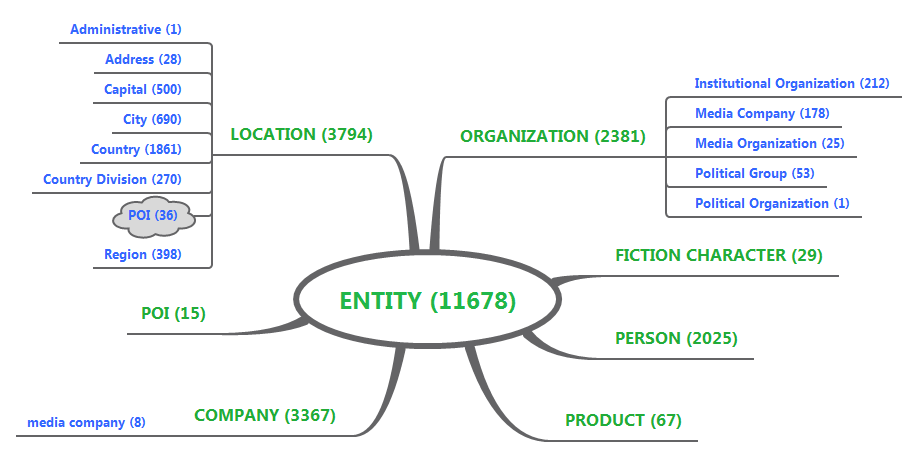
\includegraphics[scale=0.4]{images/comparo-FTB6/entities}
\caption{La hiérarchie des types du FTB annoté en entités nommées}
\label{fig:ftb6-hierarchy}
\end{figure}

\begin{table}[ht!]
\centering
\begin{tabular}{|c|c|c|c|}
\cline{2-4}
\multicolumn{1}{c|}{ } & Entrainement & Développement & Test \\
\hline
Phrases    & 9881 & 1235 & 1235 \\
Entités    & 9235 & 1271 & 1173 \\
\hline
\end{tabular}
\caption{Une vue d'ensemble du FTB annoté en entités nommées}
\label{tab:ftb6-overview}
\end{table}

\begin{figure}[ht!]
\begin{helvetica}
\small
$[$...$]$ \textcolor{teal}{[ORGANIZATION France 3]}, \textcolor{green!50!black}{[COMPANY Canal Plus]}, \textcolor{teal}{[ORGANIZATION M6]}, documentaire sur \textcolor{teal}{[ORGANIZATION Arte]}.\\
$[$...$]$ le président de la république du \textcolor{red}{[LOCATION Chili]}, \textcolor{blue}{[PERSON Patricio Aylwin]}, $[$...$]$ \\
$[$...$]$ les théâtres du \textcolor{purple}{[POI Vieux-Colombier]} et de la \textcolor{purple}{[POI gaîté-lyrique]} $[$...$]$ \\
$[$...$]$ ancien propriétaire de la marque \textcolor{gray}{[PRODUCT Reebok]}, $[$...$]$ \\
"Nous étions \textcolor{orange}{[FICTION\_CHARACTER Tintin]} bien avant tout le monde $[$...$]$
\end{helvetica}
\caption{Des exemples d'entités corpus FTB}
\label{fig:FTB-examples}
\end{figure}

Par rapport à l'étendue des entités, sont annotées toutes les entités qui étaient valables à l'époque où les articles journalistiques étaient écrits (par exemple, l'URSS existait encore à cette époque). Cela implique que les pays désormais disparus, comme l'URSS et la Tchécoslovaquie, sont annotés dans le corpus car ils existaient encore à l'époque. Cela signifie que la plupart des systèmes à base de règles risquent de commettre des erreurs sur ces entités qui sont généralements filtrées.

La particularité du FTB annoté en entités nommées est qu'il dispose également du référencement des entités nommées selon une base de données, ici Aleda \citep{sagot2012aleda}, extraite automatiquement depuis Wikipedia et Geonames. Le FTB annoté en entités nommées permet donc non seulement d'effectuer de la reconnaissance d'entités nommées, mais également de l'entity linking.

\end{document}